\chapter{Cardiac Electrophysiology}
\label{chap:cardiac_electrophysioloy}

The heart generates electric currents which produce potential fields in the
body. There are situations in which there is electrical activity; yet the heart
doesn't contract (e.g. atrial fibrillation or ventricular fibrillation). This is
known as {\bf pulseless electrical activity} (PEA), leading to loss of cardiac
output. The condition of sudden arrhythmias death syndrome (SADS) can be
inherited, it's important to evaluate you the signs of these disease if one of
your relative died of SADS. This can be the result of ion channelopathies, e.g.
LQTS or CPVT, or sudden cardiac death during sleep caused by sodium channel LQTS
or Brugada syndrome (Sect.\ref{sec:brugada-syndrome}). Different strategies for
medical examination \footnote{\url{http://www.sads.org.uk/cardiac_tests.htm}}.

To measure pumping ability, we use different techniques, e.g.
{\bf ultrasound-based (echocardiography)}, and {\bf nuclear medicine test}.
Echocardiogram (using ultrasound wave) can detect structural change (or damage)
in the heart, e.g. valve prolapse, cardiomyopathy (e.g. inefficient pumping
function of the heart). {\bf Cardiomulmonary exercise test} analyze the
efficiency of the heart muscle, by measuring the amount of oxygen your body use,
e.g. breathing into a device during exercise. If the efficiency is low, it may
suggests you have cardiomyopathy. Even with normal structure, the electrical
activity can be abnormal. This can be detected using {\bf ECG} which is the
important non-invasive technique to measure heart's behavior. To record ECG data
for a continuous longer period of times (e.g. 24 hours, and upto 7 days for a
digital one) that can help to symptom detection and lead to earlier clinical
decision, {\it Holter device} is used (attaching 4-6 electrodes on the body).
{\bf Cardiomemo} is more sophisticated version of Holter device, without using
electrodes, i.e. when you feel the symptoms, you activate the device and put it
on the chest and it will record the data. For infrequent symptom, it will be
difficult to assess and record it. Thus, a {\bf reveal} device is used
(developed by Bio); it is an implantable continuous monitoring device with an
installed algorithm to detect atrial fibrillation (AF).
\begin{itemize}
  \item  Reveal XT ICM (XT Insertable Cardiac Monitor) device: with battery can
  last upto 2 years, and can detect AF with sensitivity 96.1\%, and can confirm
  the absence of AF in patients without AF (negative predictive value NPV) at 97.4\%.
\footnote{\url{http://www.innovatingforshd.com/downloads/Role-of-Reveal-in-AF-Monitoring-Brochure.pdf}}

  \item Reveal LINQ ICM: the smallest heart
  monitor available (1/3 of the size of an AAA battery), battery work for upto 3
  years, placed under the skin of your chest (in a simple outpatient procedure), and is MRI safe, and improved AF detection with risk of false positive (FP)
  reduced, Fig.\ref{fig:Reveal_LINQ_ICM}
  \url{http://www.medtronic.com/patients/fainting/device/our-insertable-cardiac-monitors/reveal-linq-icm/}
\end{itemize}
The data can be transmitted wirelessly to the phone app or to the doctor for
further investigation.

\begin{figure}[hbt]
 \centerline{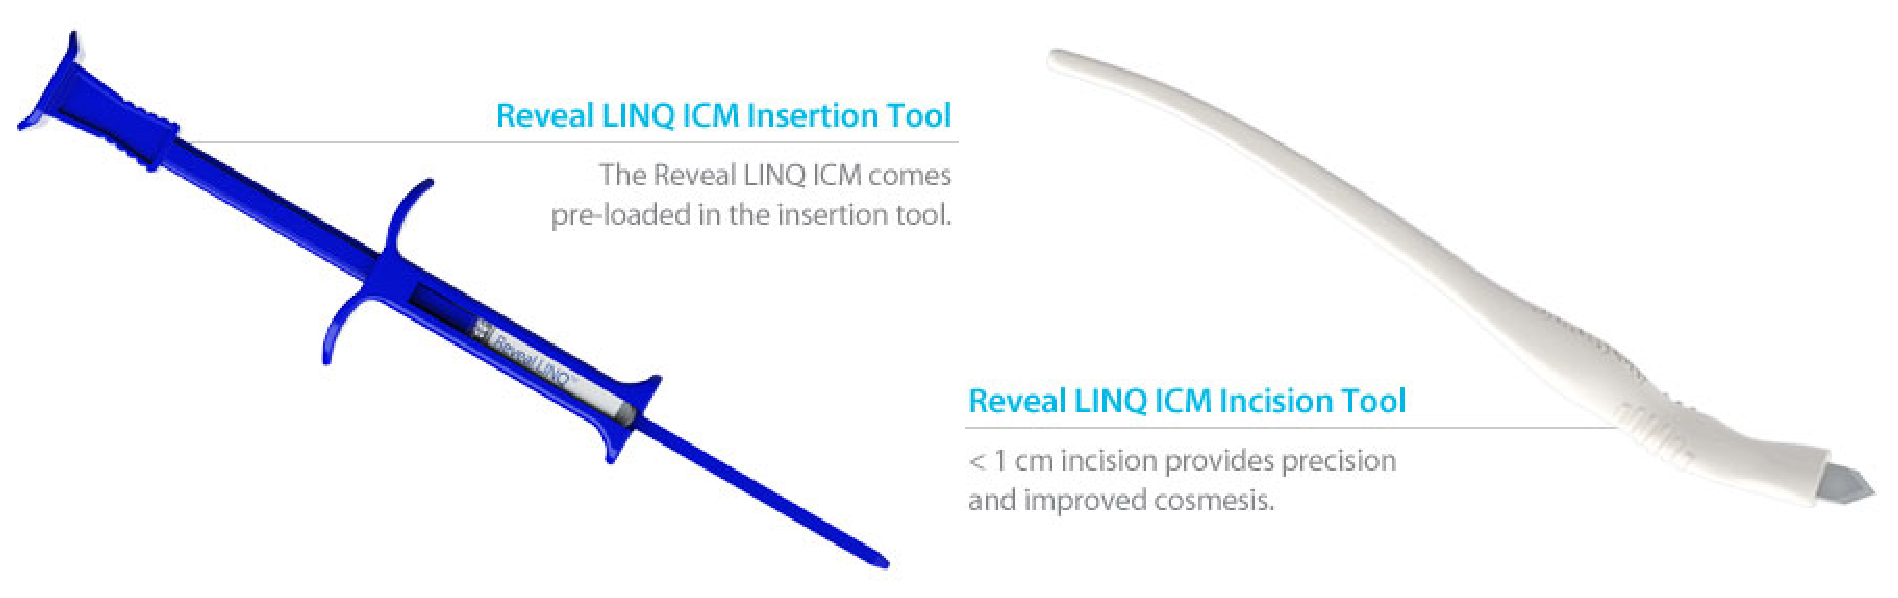
\includegraphics[height=5cm]{./images/Reveal_devices.eps}}
 \caption{Techniques to insert Reveal LINQ ICM device
 \footnote{\url{http://www.medtronicdiagnostics.com/us/cardiac-monitors/reveal-linq/cardiac-monitor-procedure/index.htm}}}
\label{fig:Reveal_LINQ_ICM}
\end{figure}

Another type of test is {\bf Genetic testing}. As most inherited conditions
can lead to SADS, the ability to detect mutations of specific genes is important
to make diagnosis, using DNA sample. However, this is still at an early stage as
we don't have complete knowledges of genes involved in all conditions. Also,
many genetic variations are found that not necessary cause any diseases.

{\bf Tilt-table testing} is used to identify common conditions that can cause
blackouts, e.g. Vasovagal syndrome (affect young girls, but very low risk of
causing sudden death). As the symptom is very much similar to the rare and
potential life-threatening conditions (e.g. channelopathies), it's important to
know the cause of blackouts. How? you lie flat on the table, and the system
measure blood pressure, pulse, ECG; and then tilt the table to an angle 60-75
degrees, and continue monitoring. If nothing happended, a spray of substance
called GTN is given to stimulate the process and monitor for 10-15 minutes. If
your blood pressure falls at the time you suffer the change, then you have
Vasovagal syndrome or a related condition. The process takes about 45 minutes.

The importance of linking ECG to the heart activity is to extend the clinical
value of interpreting ECG data. To detect subtle variation, which can be useful
for diagnosing Brugada syndrome, PCCD or ARVC, the ECG from an average of at
least 250 heartbeats are calculated. Exercise ECG is the ECG recorded during
exercise, which can be used to detect characteristics of LQTS or CPVT.

Theoretical cardiology deals with studying the potential distribution over the
surface of the torso produced by an internal time-varying source (dipolar,
quadrupolar, etc.) to provide an insight into heart behavior.  Early studies
used theoretical analysis with the heart is represented as a single
fixed-location dipole (see explanation later), and the torso as
infinite homogeneous, isotropic, resistive, linear medium in different settings
or a finite homogeneous medium of spherical or prolate spheroidal shape.
\citep{okada1956}.
\begin{enumerate}
  \item a centric dipole inside 2D equilateral triangle
  \item a centric dipole inside a sphere
  \item an eccentric dipole inside sphere
  \item a centric dipole in an infinite-length circular cylinder
  \item a centric dipole in a finite-length circular cylinder
  \item an eccentric dipole in a prolate spheroid
  \item a eccentric dipole in a finite-length circular cylinder
\end{enumerate}

In ECG calculating, one calculate an arbitrary source distribution
in a medium containing regions of different conductivity the complete potential
distribution on an irregularly shaped external surface (i.e. torso), subject to
the boundary condition that the generated currents be tangential to the external
boundary and continuous through all internal interfaces between media of
different conductivity.

Later approaches using computer can assume more complex geometries which is a
closer representation to human physiology with time-dependent sources (e.g. the
heart) embedded within an inhomogeneous conducting (the body) and dielectric
medium of irregular configuration \citep{barnard1967a}. The first comprehensive
mathematical study of relating the electrical activity within the heart to the
time-varying potential distribution on the body surface was done by
\citep{gelernter1964}.

\section{Dipoles and Magnets}

An electric charge generate around itself an {\bf electric field} $\mathbf{E}$.
Another charge when comes closer to this charge can be expelled or drawed
depending on the side (negative/positive) between the two charges. The strength
of the electric field depends on the electric charge, and is represented by
\textcolor{blue}{force per unit charge} (Newton/Coulomb or Volts/metre).
When an electric charge moves, it create a {\bf magnetic field} $\mathbf{B}$.
The strength of the magnetic field depends on both the electric charge and its
speed; and is represented in unit of Gauss or Tesla. The electric field can be
{\it monopole} or dipole; while the magnetic field must be dipole.
Both the electric field and magnetic field of a single source are related by
{\bf Maxwell's equation} (a set of PDEs).


The flow of electric current down a conducting wire is due to the moving of
electrically charged particles (which is, in most cases, electrons). For the net
charge density in the wire is zero (completely neutral), there must be
stationary charges which is, in most cases, {\it atomic nuclei}. If we put two
wires closed to each other, they can expel or attract one another if the
currents is in the opposite or the same direction, respectively. It means the
moving charge, even in a neutral wire, generate a force surrounding it. 
If we double the current in one wire, the force is double.

The {\bf magnetic field} created by the electric currents is a series of
concentric circular loops in the plane perpendicular to a current carrying wire,
Fig.\ref{fig:current_magnetic_field}. The direction of the circulation around
the magnetic loops is determined by the right-hand rule (use the thumb pointing
toward the direction of the current, and the direction of the motion of the
other fingers is the direction of the circulation).

\begin{figure}[hbt]
  \centerline{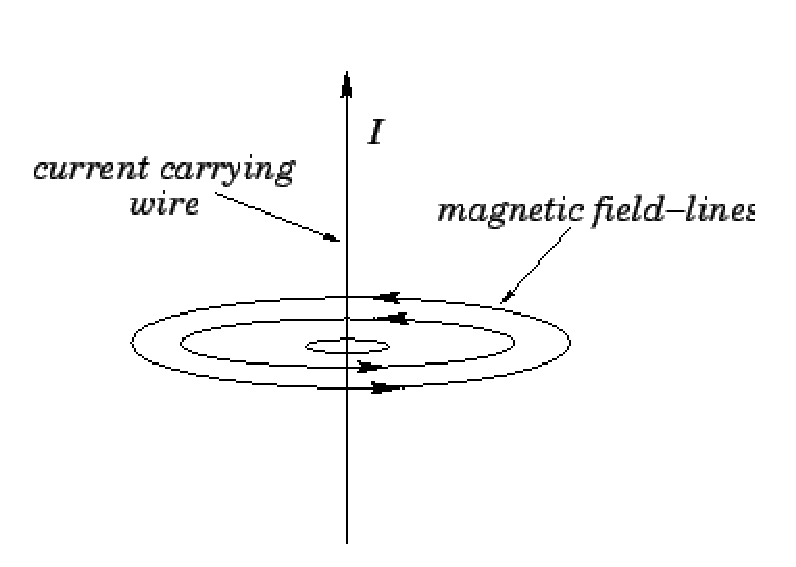
\includegraphics[height=7cm,
    angle=0]{./images/current_magnetic_field.eps}}
  \caption{Magnetic field}
  \label{fig:current_magnetic_field}
\end{figure}

When another charge $q$ moves with velocity $v$ in the magnetic field created by
an electric current, it experiences a force
\begin{equation}
\vec{F} = q \frac{\vec{v}}{c} \times \vec{B}
\end{equation}
with $c$ is speed of light. This is known as {\bf Lorentz Force Law}.
Since the current also consists of freely moving
electric charge, so the magnetic field also exert a force upon the flowing
current. So the entire wire feels a force equal to the sum of the forces acting
upon individual moving charge on the wire.

The magnitude of the electric current is [number of Coulombs (which past through
a given point) per second]. Assuming each charge has $q$ (Coulombs), moving with
a velocity $v$; so all the charges contained in the cylinder of cross-sectional
area $A$ and the length $v$ flow past a given point after one second. The
magnitude of the current is $\eta.A.v.q$ with $\eta$ is the density of the
charges. The direction of current is the same as the direction of the motion of
charges, so the vector of current is
\begin{equation}
\vec{I} = \eta.A.q.\vec{v}
\end{equation}


The current flowing through the cross-section $A$ of a conductor is the amount
of transferred charge$\Delta Q$ per unit of time [Ampere=Coulomb/sec].
\begin{equation}
I = \frac{\Delta Q}{\Delta t} = \frac{dQ}{dt}
\end{equation}
The current density $\vec{J}$ is a vector and the current $I$ is the flux of the
current density $\vec{J}$.
\begin{equation}
I = \int\int_S \vec{J} .ds
\end{equation}

The current density (A/m$^2$) has $J_n$ normal component
\begin{equation}
\begin{split}
J_n = \rho_v . v \\
J = \rho_e v_e + \rho_p v_p = (-\rho_e \mu_e + \rho_p \mu_p) E = \sigma. E
\end{split}
\end{equation}
with $p\equiv h,i$. The {\bf specific conductivity} $\sigma$ (S/m =
($\Omega \times $m)$^{-1}$) depends on the free-charge density and its mobility.
The charge density depends on the number of charged particles per unit volume
(number density), i.e. $\rho_e = -e N_e$ ($e \approx 1.6022\times 10^{-19}$(C)).
\begin{equation}
\begin{split}
\sigma_\text{semi} = ( N_e\mu_e + N_h \mu_h) e \;\;\;\; \text{semiconductor} \\
\sigma_\text{metal} = N_e \mu_e  \;\;\;\; \text{metal}
\end{split}
\end{equation}
with pure semiconductor then $N_e = N_h$, Fig.\ref{fig:specific_conductivity}.

\begin{figure}[hbt]
  \centerline{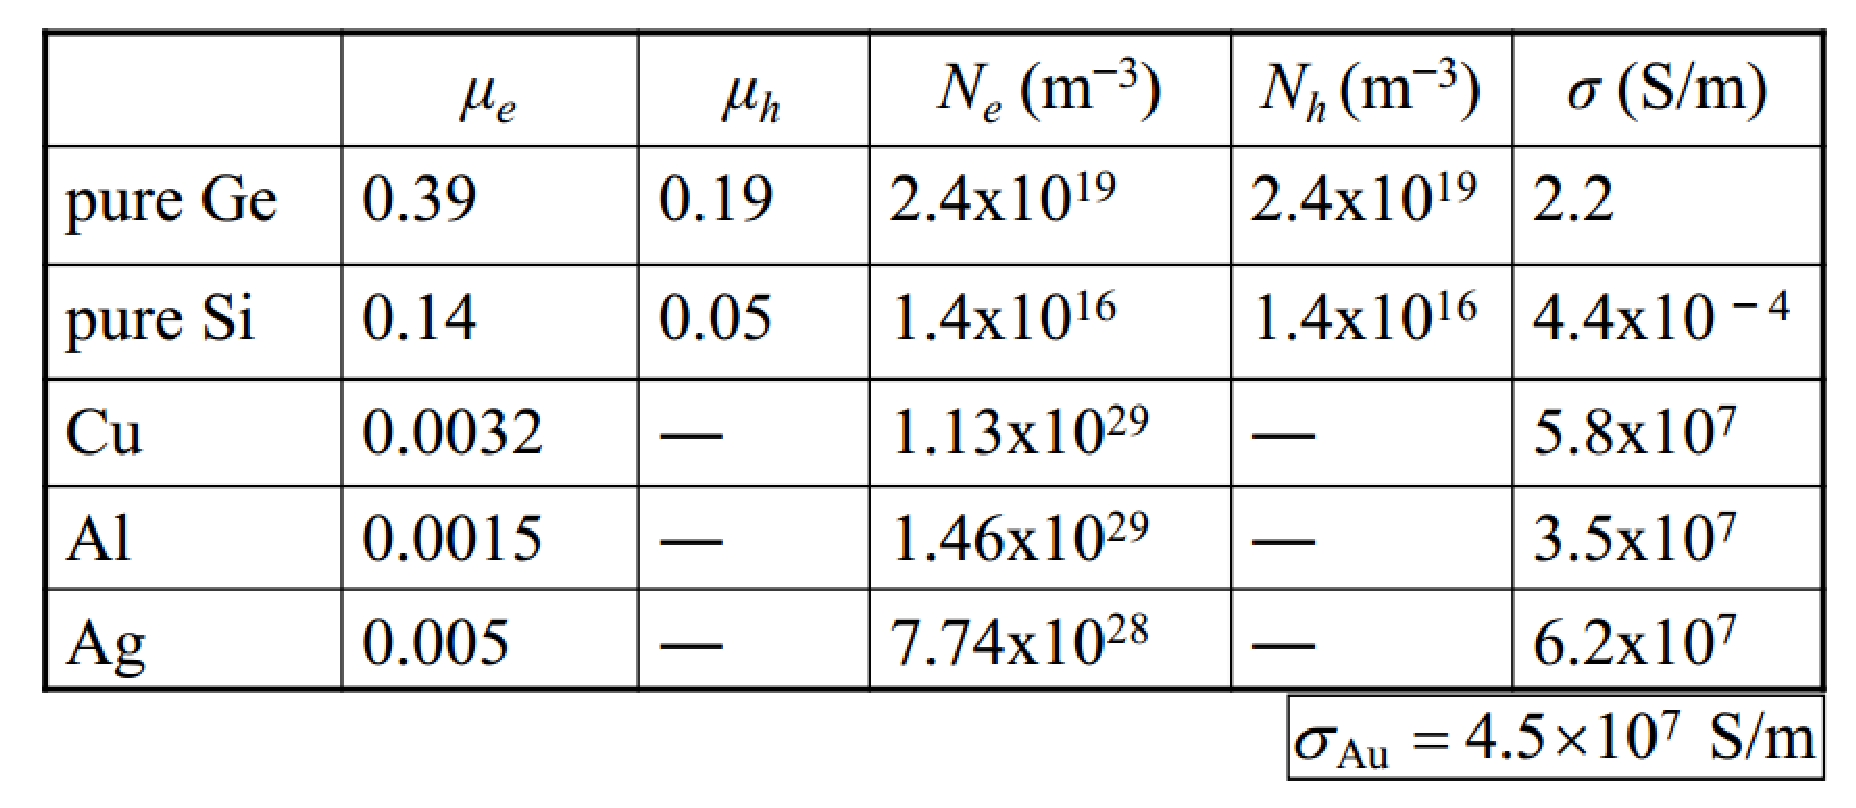
\includegraphics[height=5cm,
    angle=0]{./images/specific_conductivity.eps}}
  \caption{Number densities, mobilities, and conductivities of some conductors}
  \label{fig:specific_conductivity}
\end{figure}

So, Ohm's law in point (differential) form is
\begin{equation}
J = \sigma E
\end{equation}
In cellular electrophysiology, the equivalent form for intracellular is
\begin{equation}
J_i = \sigma_i V_m
\end{equation}
In circuits, the equivalent form is
\begin{equation}
I = J.s = \sigma .s. E = \sigma\frac{s}{l}V
\end{equation}
with $G=1/R = \sigma\frac{s}{l}$. 

The charge velocity in a conductor depends on the charge {\it mobility} which
in general depends on $\mathbf{E}$ (non-linear conductor)
\begin{equation}
v_e = -\mu_e . \mathbf{E}
\end{equation}
NOTE: 
\begin{enumerate}
  \item metals support electrons movement
  \item semi-conductors support both electron and hole movement
  \item most electrolytes support both electron and ion movement
  \item general plasmas support both electron and ion movement
\end{enumerate}


% 
% 
% {\bf Lorentz Force Law}: a charge moving in a
% magnetic field expriences a force
% \begin{equation}
% \vec{F} = q\vec{v}\times \vec{B}
% \end{equation}

\section{ECG explained}

The first ECG was published by Augustus D. Waller in 1887. He measured ECG from
his bulldog Jimmy with his paws in buckets of saline. The conducting solutions
in the buckets serve as electrodes. A device connected to the 'electrodes' to
record the potential difference. The recorded signal was seen to pulsate in
rhythm with Jimmmy's heart rate. Waller then presented the evidence to support
the idea that the recorded potential differences is the result of the electrical
activity of the heart. To do this on human, Willem Einthoven used the
galvanometer to record the potential difference at 3 limbs, i.e. giving 3
potential differences. He called lead I (potential difference left
hand-right hand), lead III (potential difference left leg-left hand), lead
II (potential difference left leg-right hand). This is called {\bf bipolar
lead}, as it records the potential difference between 2 point electrodes. As you
can see the direction of base-apex (heart-vector) in the ventricle is the
direction of lead II. So, lead II signal is quite commonly used, as shown in
Fig.\ref{fig:ECG_ideal}.  The directions of the three leads were chosen so that
a normal activation pattern gives a positive R-wave in all three leads.

The sign of the ECG signal depends on how we put the electrodes (+) and (-). To
understand the morphology of ECG, only one biophysics fact we need to remember:
If the wavefront of deplarization travel toward (+) electrode (i.e. electrode
attach to the (+) terminal) and away from the (-) electrode, a {\it
positive-going deflection} will result; otherwise, a negative-going deflection
will result. Also, if the depolarization wavefront travels perpendicular to the
axis, then an iso-electric line or a biphasic deflection will occur.

There can be multiple electrode pairs that we put on the body surface, each pair
form an axis, and the signal recorded on that pair is the votage recorded
projected on that axis, with the vector represent the direction and amplitude of
depolarization at each time.
Lead II on Einthove's ECG is to put the (-) electrode on the SA-node direction
(e.g. the right-hand in human or right fore-leg in animal), and the (+) on the
front toward the septal of the heart (i.e. the left leg in human or left hind
leg in animal). This is aka the {\bf heart's axis}.


P-wave reflect the depolarization from SA node to AV node on the atria. The
delayed in the AV node is reflected as an iso-electric (i.e. zero-voltage
period) just after P-wave. A typical ECG recorded on leak II is given in
Fig.\ref{fig:ECG_ideal}. PR-interval - the time from the onset of the P-wave
until the start of the QRS-complex, is the time taken from initiation of atrial
depolarization to the onset of ventricular depolarization. In human, PR-interval
is between 0.12sec to 0.20 sec. A prolonged PR-interval means there is a defect
in the conduction in the atria and AV node.

\begin{figure}[hbt]
  \centerline{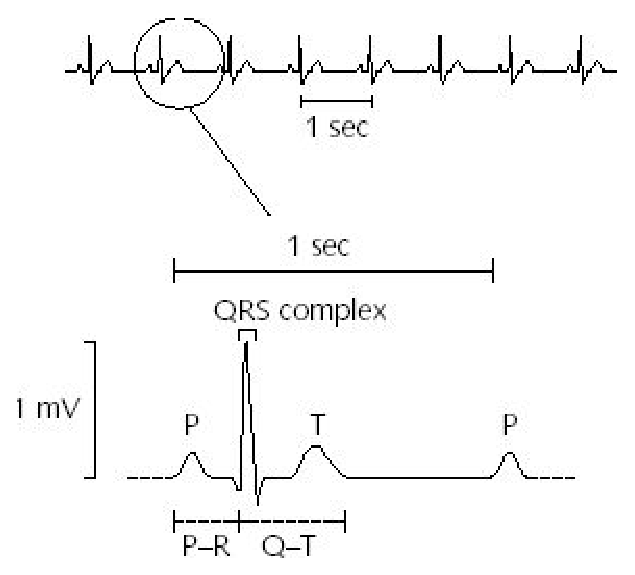
\includegraphics[height=5cm,
    angle=0]{./images/ECG_ideal.eps}}
  \caption{Ideal ECG signal on lead II}
  \label{fig:ECG_ideal}
\end{figure}

After the delay in AV node, the signal propagate very fast through the His
bundle and then the bundle branches, Purkinje fiber and cause uniformly
contraction in the ventricle. This explains a short QRS-complex (0.06sec to
0.1sec). A prolonged QRS-complex means there is a defect in the Purkinje fiber
system or some parts in the ventricle.

\textcolor{red}{Why Q-wave is negative in ECG?}: Q-wave represent {\it septal
depolarization}, i.e. move from left-to-right.
Septum is the first ventricular muscle to be activated in the interventricular
septum, then travel down to the His bundle and finally to the Left and
Right bundle branches. Q-wave is negative as  the Left bundle branches get
depolarized slight before Right bundle branches. Thus, the depolarization
get recorded first from left, then to right.

\textcolor{red}{Transmural depolarization (R-wave)}: even though ventricular
walls on both side depolarized uniformly, the endocardial surface being activated before
the epicardial surface. This generate R-wave. The reason is that left
ventricular wall is thicker than that of right ventricle; even after the
depolarization of a large part of the right ventricle, the activation of the
left ventricle free wall continues. During this time, there is no compensate
electric forces from the right chamger, the resultant vector reaches the maximum
in this phase and point leftward. The depolarization front continue propagation
along the left ventricular wall toward the back of the heart. The surface area
of unactivate regions continues to decrease during the time, then the magnitude
of the heart vector also decrease until the whole ventricle muscle is
depolarized. The last part to depolarize is the basal region of the
left ventricle and right ventricle.

\textcolor{red}{S-wave}: a few small area of the ventricles are activated
at a rather late stage. S-wave represents late ventricular depolarization. This
is the region where the AP of ventricle travel along the outermost rim of the
ventricle. The direction is actually going up, i.e. away from the (+) electrode,
so it's going down (negative deflection).

Notice that the AP in the ventricle has a long plateau during which the voltage
gradient is almost zero. This is reflected by the iso-electric period after the
QRS-complex.

Notice atrial repolarization occurs at the same time with ventricular
depolarization; yet the signal from atria is much smaller in amplitude (as
there is less atrial muscle mass as compared to ventricle). Thus, atrial
repolarizatioin is mased by the QRS-complex.

\textcolor{red}{T-wave}: T-wave corresponds to ventricular repolarization which
take longer than depolarization, i.e. longer than QRS-complex. The question is
why repolarization but give positive T-wave has been puzzled the scientists for
several decades (Sect.\ref{sec:positive_Twave}).

\textcolor{red}{In ECG, the two important intervals (along with their shapes)
that has clinical applications are QT-interval and ST-interval}. QT-interval is
the total time for ventricular depolarization and repolarization. ST-interval is
the time between ventricular depolarization and repolarization.

As you can see in Fig.\ref{fig:ECG_3leads},
\footnote{\url{http://www.medicine.mcgill.ca/physio/vlab/cardio/ecgbasics.htm}}


\begin{figure}[hbt]
  \centerline{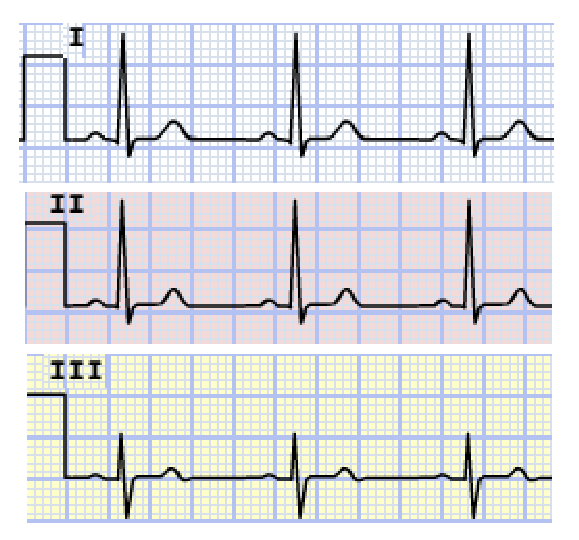
\includegraphics[height=7cm,
    angle=0]{./images/ECG_3leads.eps}}
  \caption{Different lead's orientations give different ECG}
  \label{fig:ECG_3leads}
\end{figure}

\subsection{Heart Vector}
\label{sec:heart_vector}


\begin{figure}[hbt]
  \centerline{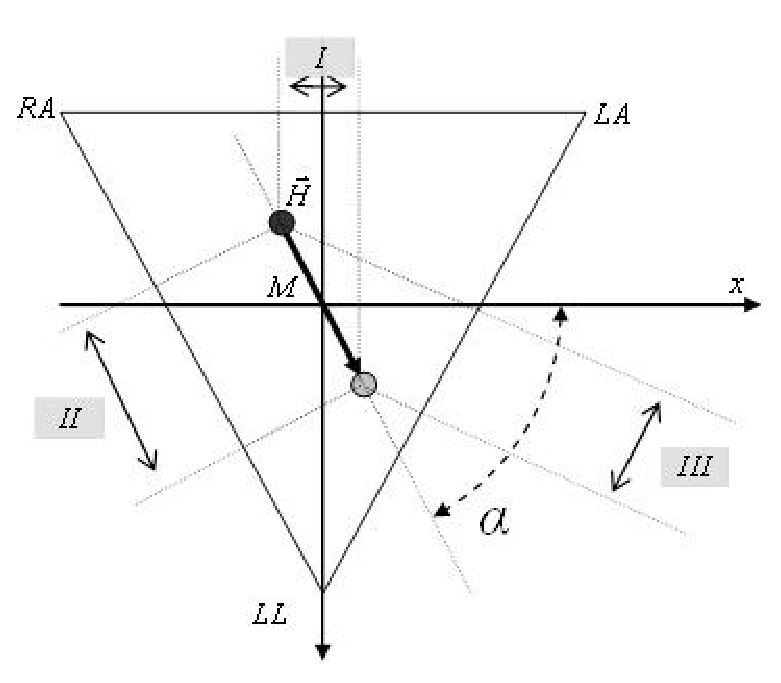
\includegraphics[height=7cm,
    angle=0]{./images/heart_vector.eps}}
  \caption{Heart vector}
  \label{fig:heart_vector}
\end{figure}

During the activation of the heart, the current sources can be approximated by a
number of dipoles, with associated dipole moments. The sum of all the dipoles
moments give a single vector describing a single dipole. This single vector is
called the {\bf heart vector}, Fig.\ref{fig:heart_vector}. The position of the
heart vector is assumed to be static, but its strength and orientation varies
during the cardiac cycle.

The potential recorded on each lead of the ECG can be interpreted as the
projection of the heart vector onto the corresponding lead-axis. So, in early
times, the signal amplitude recorded on each lead was used to construct the
heart vector, from that we can identify the changes in the activation pattern.
In 3-lead ECG, the heart vector is almost parallel to lead II, and nearly
perpendicular to lead III. So the signal from lead III is very weak, and it's
the strongest in lead II.

The 3-lead ECG developed by Eithoven, i.e. Eithoven triangle has been widely
used. All the electrical potential measured using the three leads are bipolar
leads, i.e. measured relative to some reference potentials (i.e. the ground
point). The reference point should have the potential change very little during
the course of a heart cycle. The idea is that since no electrical charge enters
or leaves the body during the heart cycle, the sum of all charges of potential
in the body must be zero. So, ideally, this zero electrode must be a remote
reference (infinity). But how to achieve this in the volume conductor of the
size of the human body with electrodes already placed at the extremities?.
Wilson {\it et al.} (1931, 1934) suggested the use of {\it central terminal} as
this reference. Ideally, one could construct a zero electrode by connecting a
large number of elecrodes, distributed over the entire body.
However, the fact is that connecting the three limb electrodes to a central
point, via 5k$\Omega$ resistor each line, is good enough to give a reference
electrode with sufficiently small variation. This is indeed the average of the
limb potential and the obtained reference potential is called {\bf Wilson
central terminal}. Nowadays, a much higher resistance is used which increases
CMRR and diminishes the size of artifact introduced by the electrode/skin
resistance.

\subsection{Why 6-lead or 12-lead ECG}

The 3-lead ECG measured the voltage when comparing the potential of one limb
lead to another. For example, the zero-electrode is RA when we calculate LA,
Table.\ref{tab:ECG_leads}. The reference point is not zero, so it's a bipolar
lead.

\begin{table}[hbt]
\label{tab:ECG_leads}
\begin{center}
\begin{tabular}{lcc}
Lead & Exploring & Zero \\
I & LA & RA \\
II & LL & RA \\
III & LL & LA \\
V1-V6 & 1-6 & RA, LA and LL \\
aVR & RA & LA and LL \\
aVL & LA & RA and LL \\
aVF & LL & RA and LA \\
\end{tabular}
\end{center}
\caption{How the potential at each lead is calculated}
\end{table}

Even though 3 leads provide many useful information, it's not enough as the
heart is not oriented in the frontal plane of the body, i.e. the plane defined
by the position of the three limb electrodes. In other words, the heart vector
is not always oriented in the frontal plane of the body. Thus, more leads have
been added to produce a more accurate picture of the condition of the heart.

As the reference point is considered as zero-potential, the Wilson central
terminal is used to construct {\bf unipolar leads}, i.e.
leads that characterie the potential changes at a single point only. The 6
unipolar leads V1-V6 were constructed by placing 6 electrodes on the front of
the chest, Fig.\ref{fig:ECG_6leads}.

\begin{figure}[hbt]
  \centerline{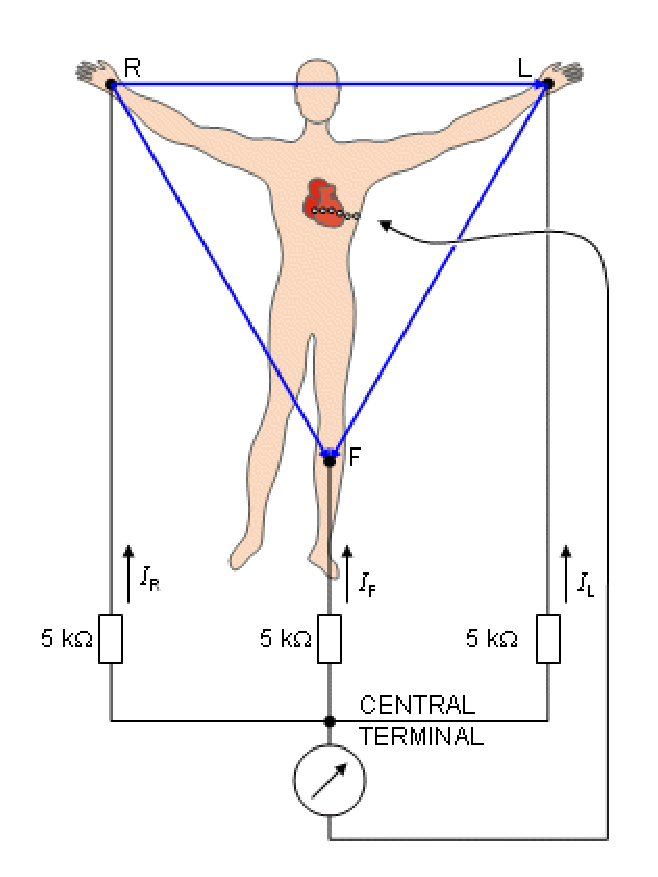
\includegraphics[height=5cm,
    angle=0]{./images/ECG_6leads.eps}}
  \caption{ECG 6 leads with the central terminal is formed by connecting three
  limb electrodes together via 5k$\Omega$. The goal is to have no current flows
  through the high-impedance voltmeter, i.e. Kirchoff's law requires
  I$_R$+I$_L$+I$_F$=0}
  \label{fig:ECG_6leads}
\end{figure}

The 3-lead and V1-V6 form the standard 9-lead ECG in 1938, with each lead is
unipolar.

In 1942, three additional leads were added by Goldberger (augmented limb leads):
aVR, aVL, and aVF. Here, the zero-electrode lead is formed by connecting only
two leads, Tab.\ref{tab:ECG_leads}. So, the voltage is defined by comparing the
potential in each of the three limbs vs. a reference defined by connecting the two other limb leads.
They are considered as unipolar leads as well, even the reference point is
constructed from 2 limbs only.

However, it's not always correct that the more leads the more useful.
There's an ongoing debate regarding the possible advantages of using additional
leads.

\subsection{Reading ECG - the inverse problem}

As a non-invasive technique, the major goal of using ECG is to provide
a diagnostic power to the underlying electrical activity of the heart. This is
known as the {\bf inverse problem}. The so-called {\bf forward problem} is to
generate ECG using the AP generated from the whole-heart computational models,
Fig.\ref{fig:ECG_explained}.

\begin{figure}[hbt]
  \centerline{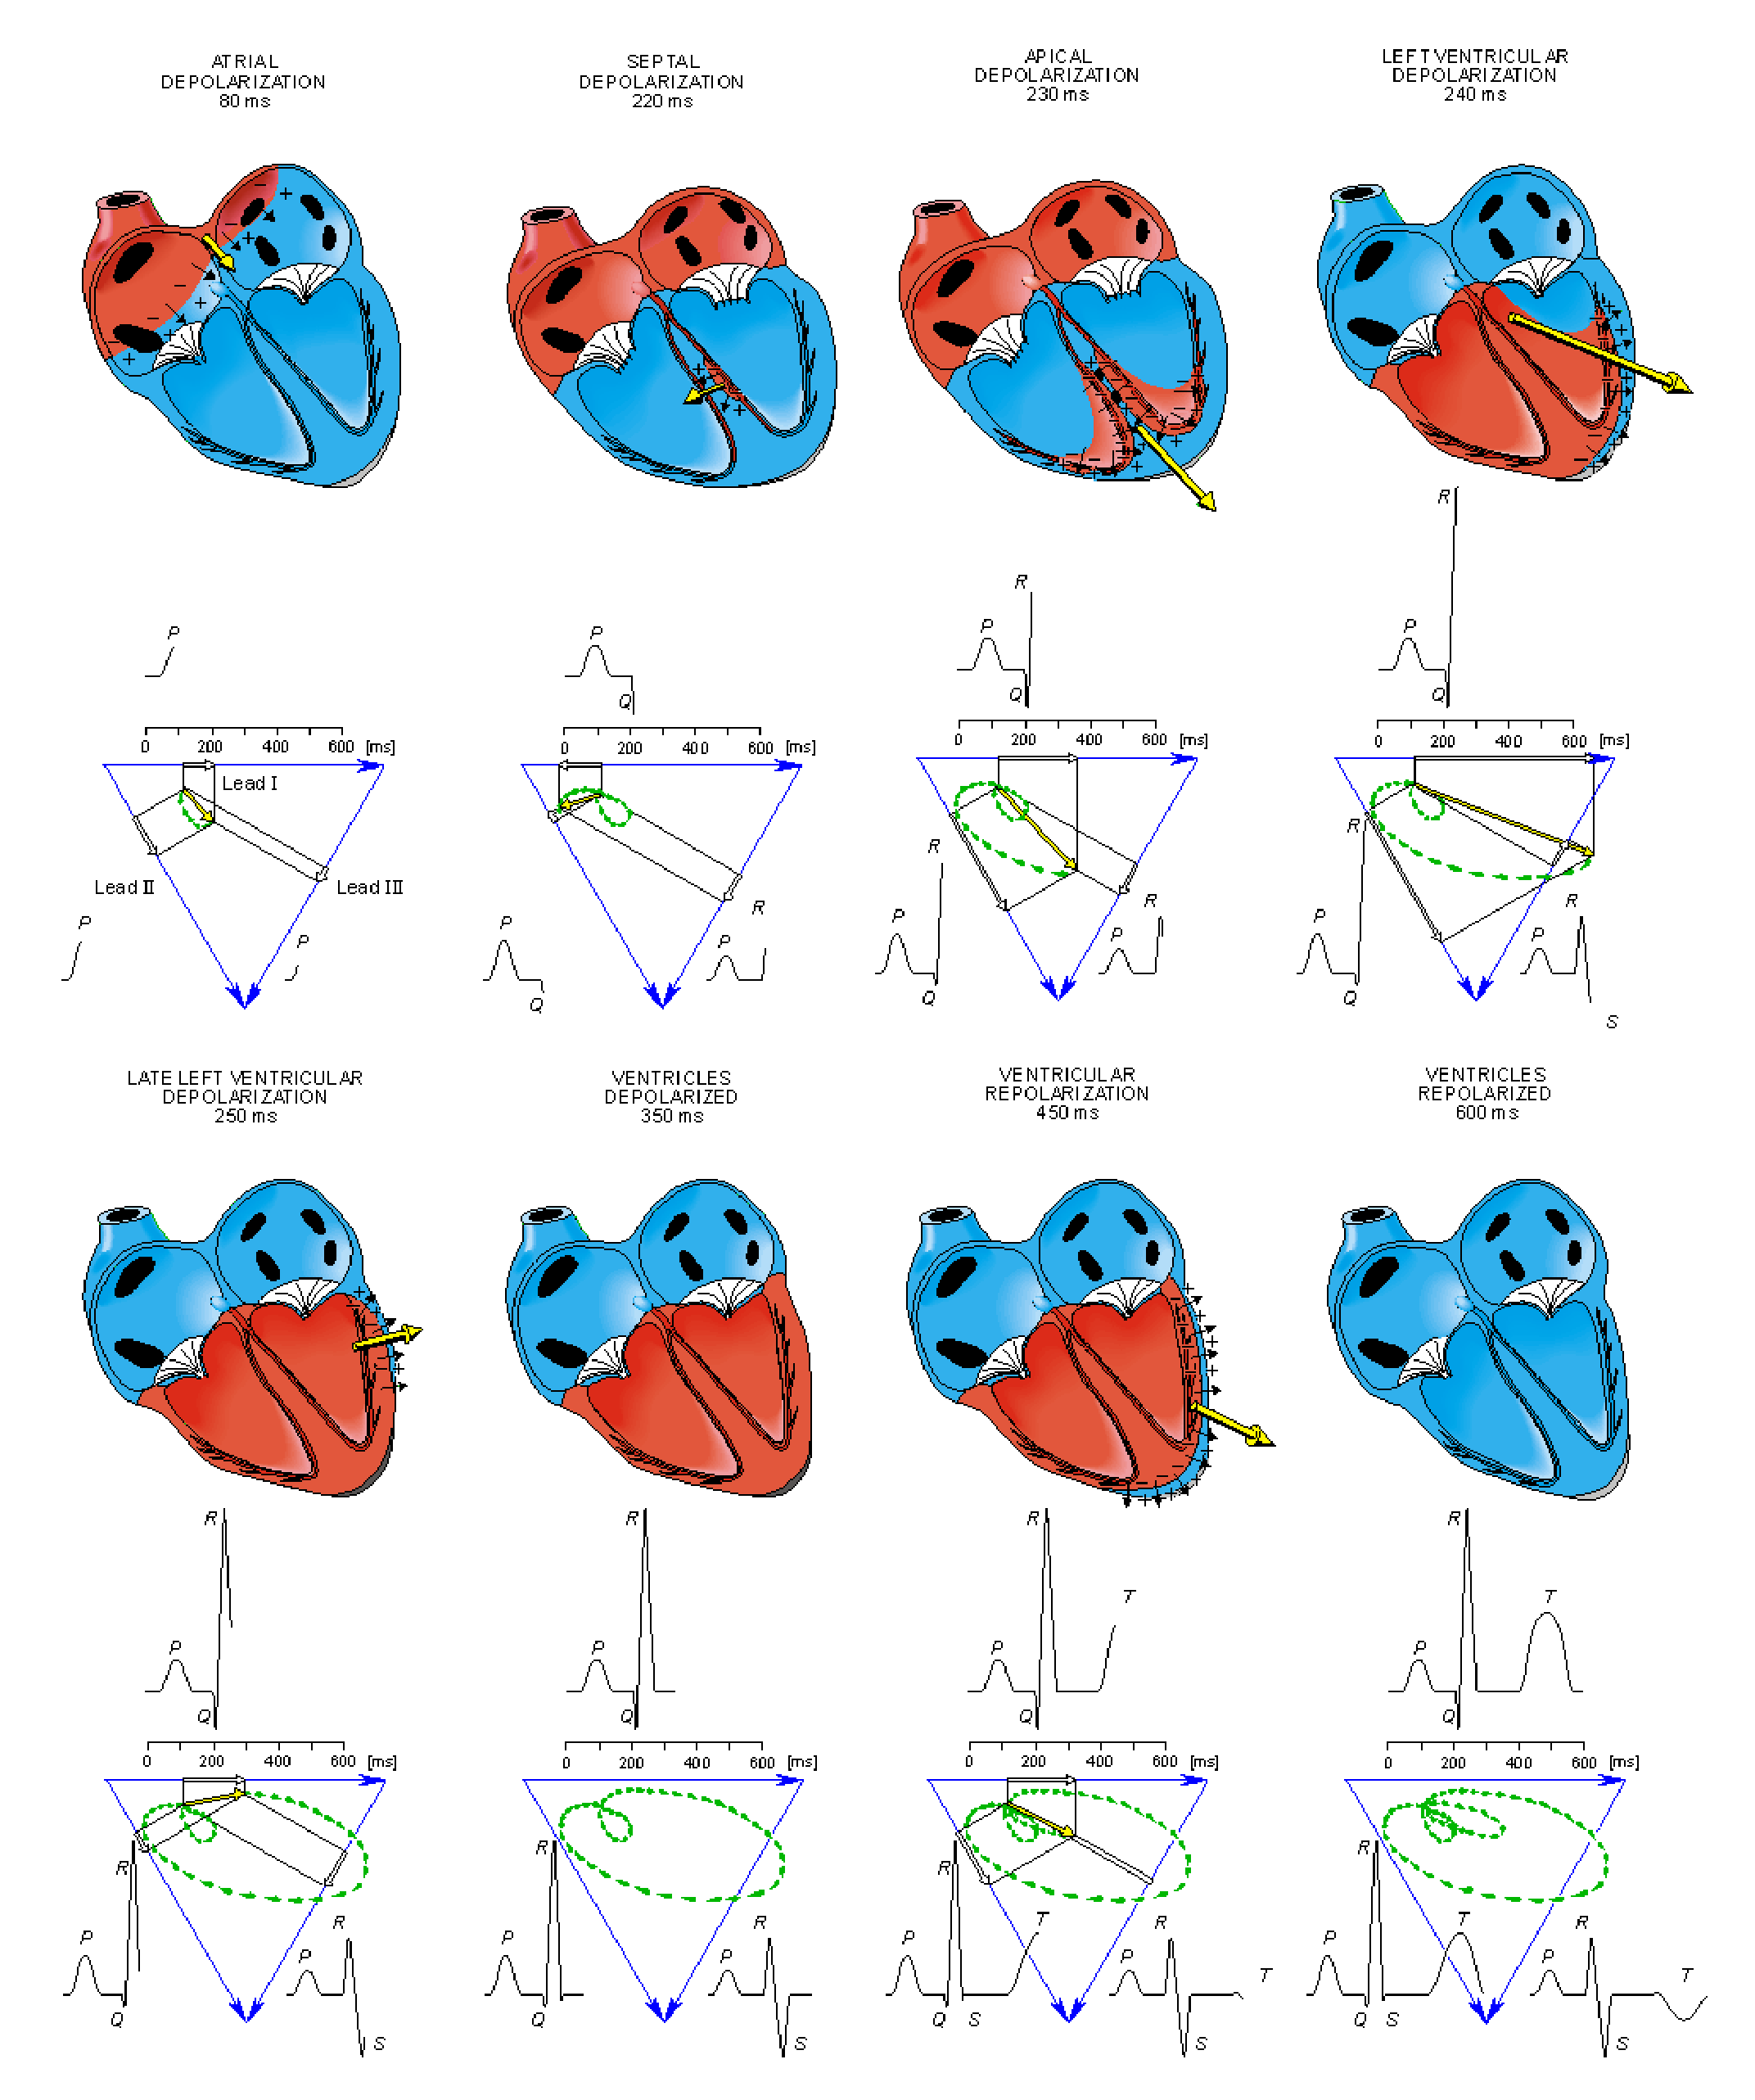
\includegraphics[height=15cm,
    angle=0]{./images/ECG_explained.eps}}
  \caption{ECG explained}
  \label{fig:ECG_explained}
\end{figure}


The abnormalities in the heart can lead to a shift in the heart vector, which
can be identified by changes in the signal amplitude recorded in each lead.
\begin{enumerate}
  \item shift in the ST segment: 
  \begin{itemize}
    \item in normal heart, it's a straight line that is on a level with
    TP-segment (the interval between T-wave and next P-wave)
    \item ischemia: a portion of the heart lacks a sufficient blood supply.
    Depending on the size and location of this ischamic area, the ST-segment can
    be shift either up or down compared to ST-segment 
  \end{itemize}
  
  \item 
\end{enumerate}



\subsection{Positive T-wave}
\label{sec:positive_Twave}


The fact that polarity of T-wave is the same as that of QRS-complex is a
challenging question. A number studies showed that this is the electrical
manifestation of ventricular repolarization sequence from the Epi- to Endo-
region that is opposite to that of ventricular activation sequence (which is
from Endo- to Epi- site). This can be explained only if the APD of Endo- region
is longer than that in Epi- site.

The change in T-wave morphologies have been linked to abnormalities in
ventricular repolarization, which plays an important role in the genesis of
arrrhythmias \citep{zhu2009}.

\section{General concepts in ECG modelling}

It can be confusing due to some terminologies which can be used by physicist's
way and engineer's way. We need to use the physicist's way.

\subsection{Dipole = heart+torso(bath)}
\label{sec:heart_dipole}

Currents in the brain is not like current through a wire, so we don't use Ampere
but we use current density (i.e. current per unit of volume). A current dipole
consist a source at the dendrite and a sink at the soma (or the other way
around, depending on whether it's an exitatory or inhibitory synapse). The
current source and sink together form a {\bf dipole}
\footnote{\url{http://kurage.nimh.nih.gov/meglab/Meg/EquivalentCurrentDipole}}.

\citep{waller1887} measured the electric field on the surface of the thorax,
Fig.\ref{fig:heart_dipole}. The result showed that the heart is a dipole with
positive pole in (A), and negative pole in (B), which can be represented in
vector form. The measurement and display the electric heart vector is called
{\it vectorcardiography} (VCG) (or vectorelectrocardiography (VECG) to separate
it from vectormagnetocardiography)
\footnote{\url{http://www.bem.fi/book/16/16.htm}}. The dipole is a source, and
the torso is a sink.


% The current dipole in cardiology consist of the heart as the source and another point in the torso as the sink.
% The distance between source and sink determine the impact that the current
% generator has on the secondary currents in the surrounding tissue.
% 
In early days, the heart was represented as a dipole source with the positive
pole placed immediately in front of the excitation wave, and a negative pole
placed immediately behind the wavefront \citep{wilson1933}. Dipole-source-based
approaches to model the heart as a single lumped-parameter description were
being used in modelling cardiac activity (Chap.\ref{chap:model-cardiac-cells}).
Since 1960s, experimental observations suggested that a single dipole cardiac
source is too simple to account for more complex cardiac waveforms
\citep{taccardi1963}. 

\begin{figure}[hbt]
  \centerline{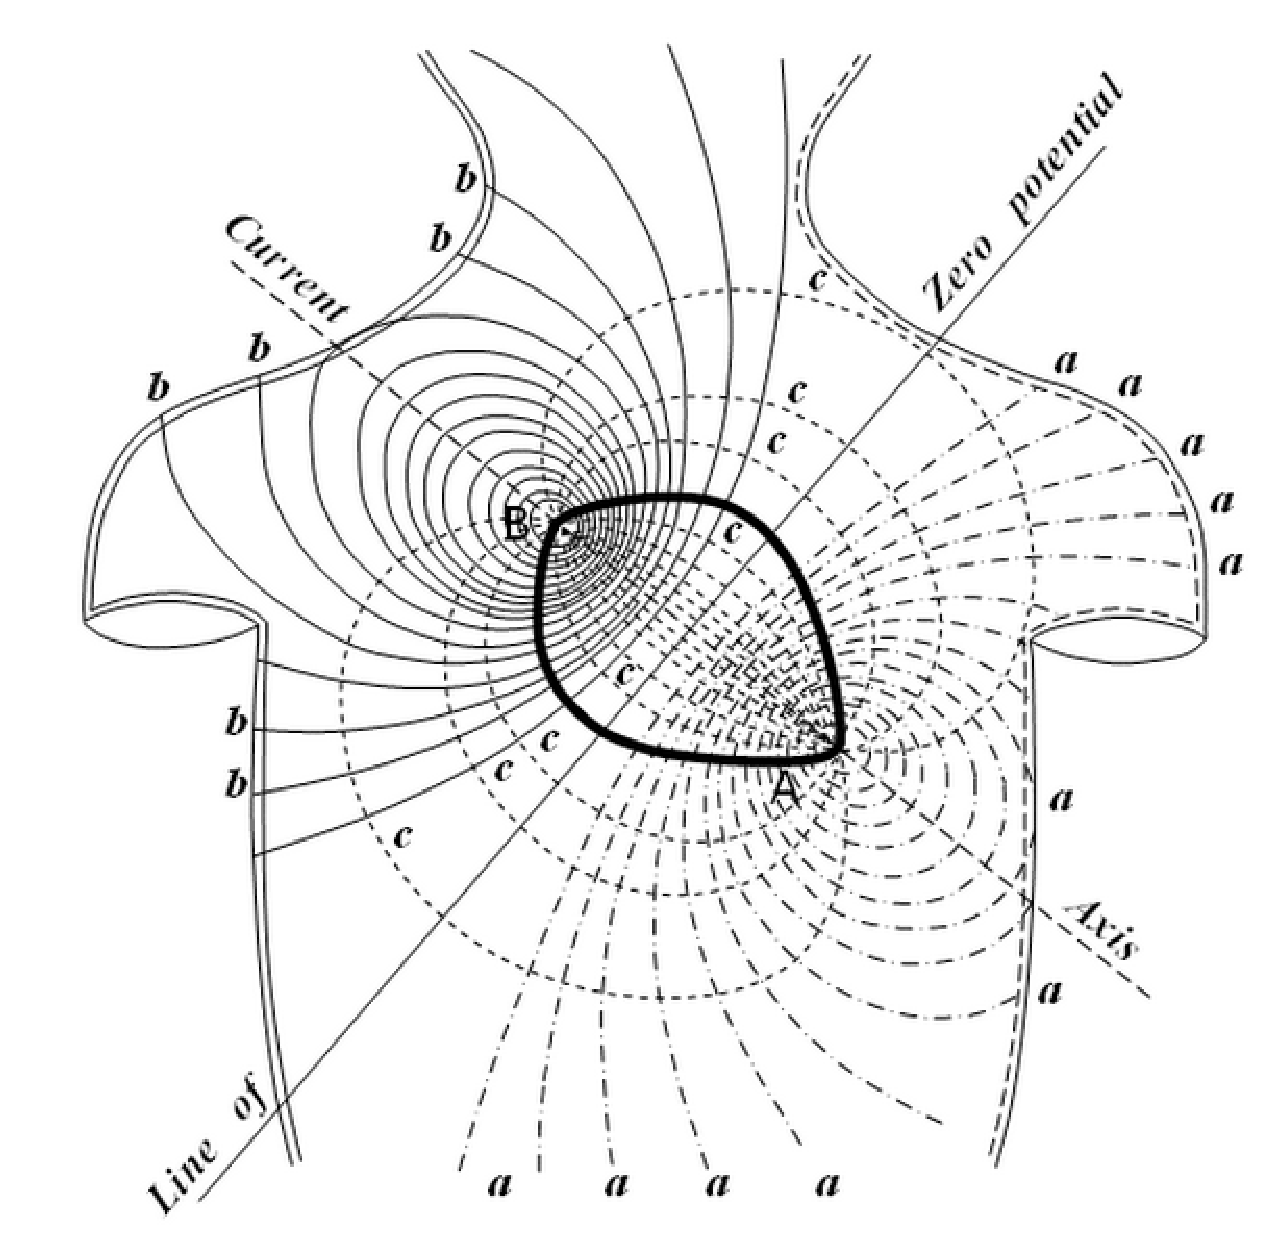
\includegraphics[height=7cm,
    angle=0]{./images/heart_dipole.eps}}
  \caption{The electric field generated by the heart on the surface of the
  thorax. The iso-potential lines are (a) and (b). These indicates the heart is
  a dipole. The curves (c) represent the current flow lines}
  \label{fig:heart_dipole}
\end{figure}

This was initiated with Eithoven's triangle.
Thus, depending on the lead position, different vectors can also be assumed. The
recorded signal is then adjusted using a given formula to give the 'correct'
estimated potential of the heart \citep{mcfee1950}. 
The heart dipole is represented by the vector
\begin{equation}
\vec{p} = \vec{i} p_z + \vec{j} p_y + \vec{k} p_z
\end{equation}
where $p_x,p_y,p_z$ are functions of time; $\vec{i},\vec{j},\vec{k}$ are unit
vectors of the rectangular coordinate system. The potential difference between
any point in the medium with the midpotential of the dipole is
\begin{equation}
V_m = \vec{c}\cdot \vec{p} 
\end{equation}
with $\vec{c}$ is a function of shape, size, and characteristics of the medium,
the position of the dipole and the position of the point in the medium that we
use to calculate $V_m$.

However, the wavefront produced by the heartbeat interpreted as a simplified
vector-projection theory that involves a centric dipole and a homogeneous
conducting sphere is not accurate enough. \citep{frank1954} proposed a new
theory which assumed (1) human body is a heterogeneous linear resistive
conducting medium, (2) the equivalent heart dipole remain fixed in position
during the cardiac cycle, (3) the distribution of current generated by the heart
on each point in the torso at a given time point: the current can be represented
as a single current dipole with direction and moment are function of the actual
current distribution. So, the medium boundary can have any shape, the electrodes
can be put anywhere, not necessarily at the apices of the triangle.


\subsection{ECG}

At the simple level, we consider a strip of muscle placed between two electrodes
attached to a volt-meter that measures the potential difference between two
electrodes (a) and (b). When a current is injected to the cells on the left side
(stimulus), an AP is generated and propagate toward the right. The volt-meter
record the potential difference between (a) and (b). The volt-meter is connected
in such a way that the recording pen moves upward when (b) is electrically
positive w.r.t. (a). By convention, the depolarizing wave move toward the
positive electrode produce produces an upward (positive) signal. 

At the realistic (more complex) level, the human torso is a 3D conductive medium
(a volume conductor) and asymmetrical that produces more complex waveforms.
However, the basic principles is the same as the 2D tissue described above.
\textcolor{red}{The heart can be depicted as a dipole} (i.e. an electric source
consisting of an assymetrically distributed electrical charge) as one region of
the myocardium is depolarized while the remaining regions are still at resting
state at any instant during the spread of a wave depolarization.

\subsection{Potential}

Given the case of a dipole in a finite-length circular cylinder,
Fig.\ref{fig:dipole_source}.  The dipole is considerred as small and is assumed
as a single point source of strength I, and the cylinder is considered as in an
infinite (up and down side) homogeneous conducting medium of conductivity
$\gamma$. 

The magnitude of the electric field $E$ created by a single point charge $Q$ at
a certain distance $r$ in vacuum is
\begin{equation}
|E| = \frac{|Q|}{4\pi\varepsilon_o r^2}
\end{equation}
NOTE: An electric field is a vector field. The force between two electric
charges $q_1, q_2$ of distance $r$ is given by Coulomb law
\begin{equation}
|F| = k_e \frac{q_1q_2}{r^2}
\end{equation}
with $k_e=\frac{1}{4\pi\varepsilon_o}$ is the Coulomb's constant.
\begin{equation}
k_e = 8.9875517873681764 \times 10^9 \text{N.m$^2$/C$^2$}
\end{equation}
We use Coulomb's law when we know the charge distribution. However, if we don't
know the distribution, e.g. in the case of (volume) conductors of the torso, we
have to use other methods, e.g. Laplace equation
\footnote{\url{http://en.wikibooks.org/wiki/Electrodynamics/Laplace's_Equation}}.

\textcolor{red}{The electric potential (voltage) produced by a current dipole
above vs. another position must satisfy the Laplace's equation and boundary
condition of zero normal derivative at the surface}.  Consider a region of the
space with charge density not zero $\rho$, the Laplacian operator $\nabla^2$ on
the electric potential over that region is defined by the Poisson equation, and
where the charge density is zero over that region, the Poisson's equation become
{\bf Laplace's equation}. 	
\begin{equation}
\nabla^2 V = \frac{-\rho}{\varepsilon_o}
\end{equation}

\begin{framed}
The electric field is related to the charge
density by the {\it divergence relationship}
\begin{equation}
\nabla E = \frac{\rho}{\varepsilon_o}
\end{equation}
with $E$ = electric field, $\rho$ = charge density, and $\varepsilon_o$ =
permitivity. The electric field is related to the electrical potential by the
gradient relationship $E=-\Delta V$. Thus, the potential is related to the
charge density by the Poisson equation:
  $\nabla^2 V = \frac{-\rho}{\varepsilon_o}$. In the charge-free medium, this
  becomes the Laplace's equation: $\nabla^2 V = 0$.

\end{framed}  

\subsection{Poisson equation, Laplacian equation}

Laplace's equation is one of the most significant equations in physics
The Laplacian operation $\nabla^2$ is the divergence of the gradient of a
scalar function. It's important to know how to solve the equation in Cartesian,
cylindrical and spherical coordinates.

Here is for rectangular coordinates (x,y,z)
\begin{equation}
\nabla^2 V= \nabla\cdot\nabla V=\frac{\partial^2 V}{\partial x^2} +
\frac{\partial^2 V}{\partial y^2} + \frac{\partial^2 V}{\partial z^2}
\end{equation}  
Here is for cylindrical polar coordinates $(r,\phi,z)$
\begin{equation}
\nabla^2 V = \frac{\partial^2V}{\partial r^2} +
\frac{1}{r}\frac{\partial V}{\partial r} + \frac{1}{r^2}
\frac{\partial^2V}{\partial \theta^2} + \frac{\partial^2V}{\partial z^2}
\end{equation}
Here is for spherical polar coordinates $(r,\phi,\theta)$
\begin{equation}
\label{eq:spc}
\nabla^2 V = \frac{\partial^2V}{\partial r^2} +
\frac{1}{r^2}\frac{\partial^2V}{\partial \theta^2} +
\frac{1}{r^2\sin^2\theta}\frac{\partial^2V}{\partial \phi^2} +
\frac{2}{r}\frac{\partial V}{\partial r} + 
\frac{\cot\theta}{r^2} \frac{\partial V}{\partial \theta} 
\end{equation}
with $\theta$ is the polar angle measured down from the north pole, $\phi$ is
the azimuthal angle, anaglogous to longitude in earth measuring coordinates.
The two latter coordinates are given in Fig.\ref{fig:coordinates}.


\begin{figure}[hbt]
%   \centerline{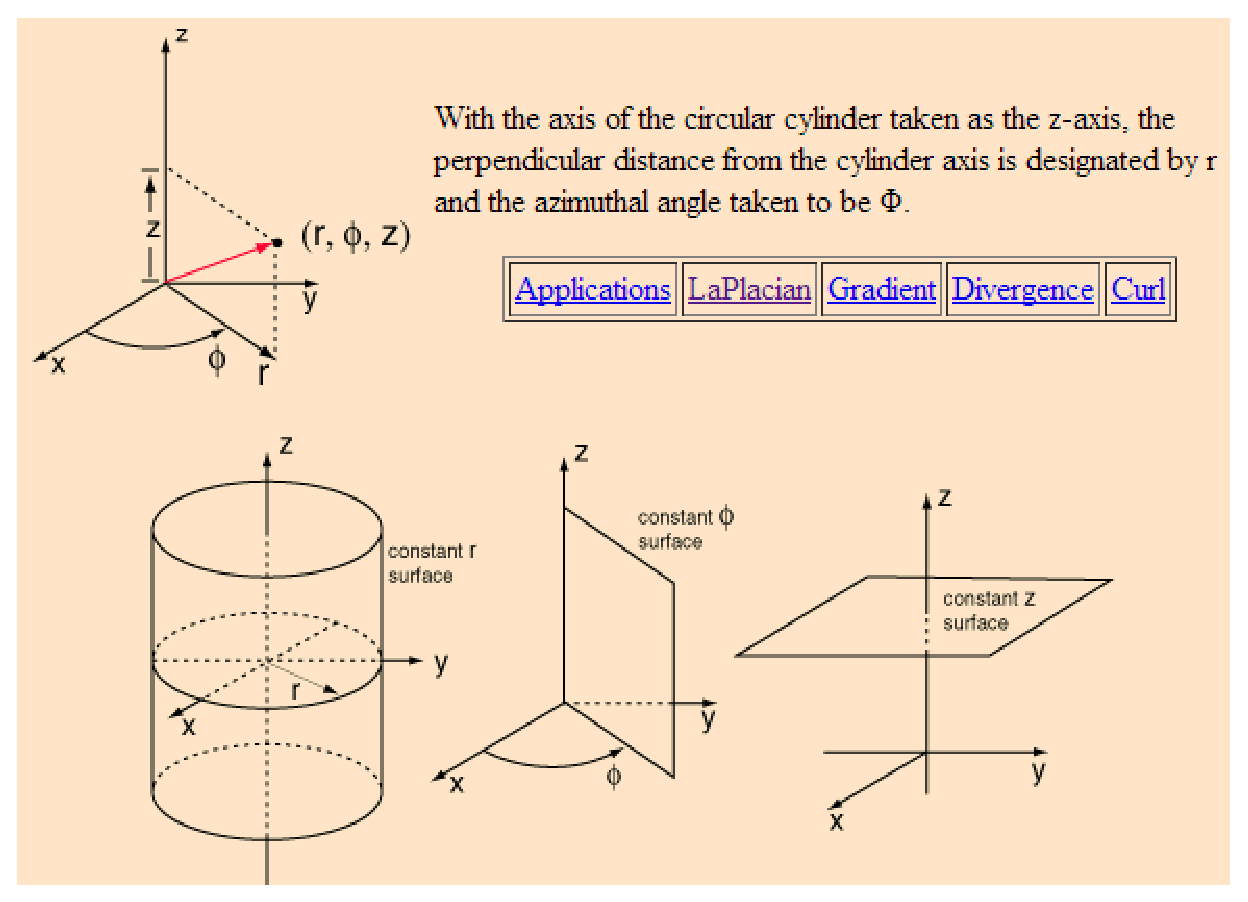
\includegraphics[height=5cm,
%     angle=0]{./images/cylindrical_coordinate.eps}}
%       \centerline{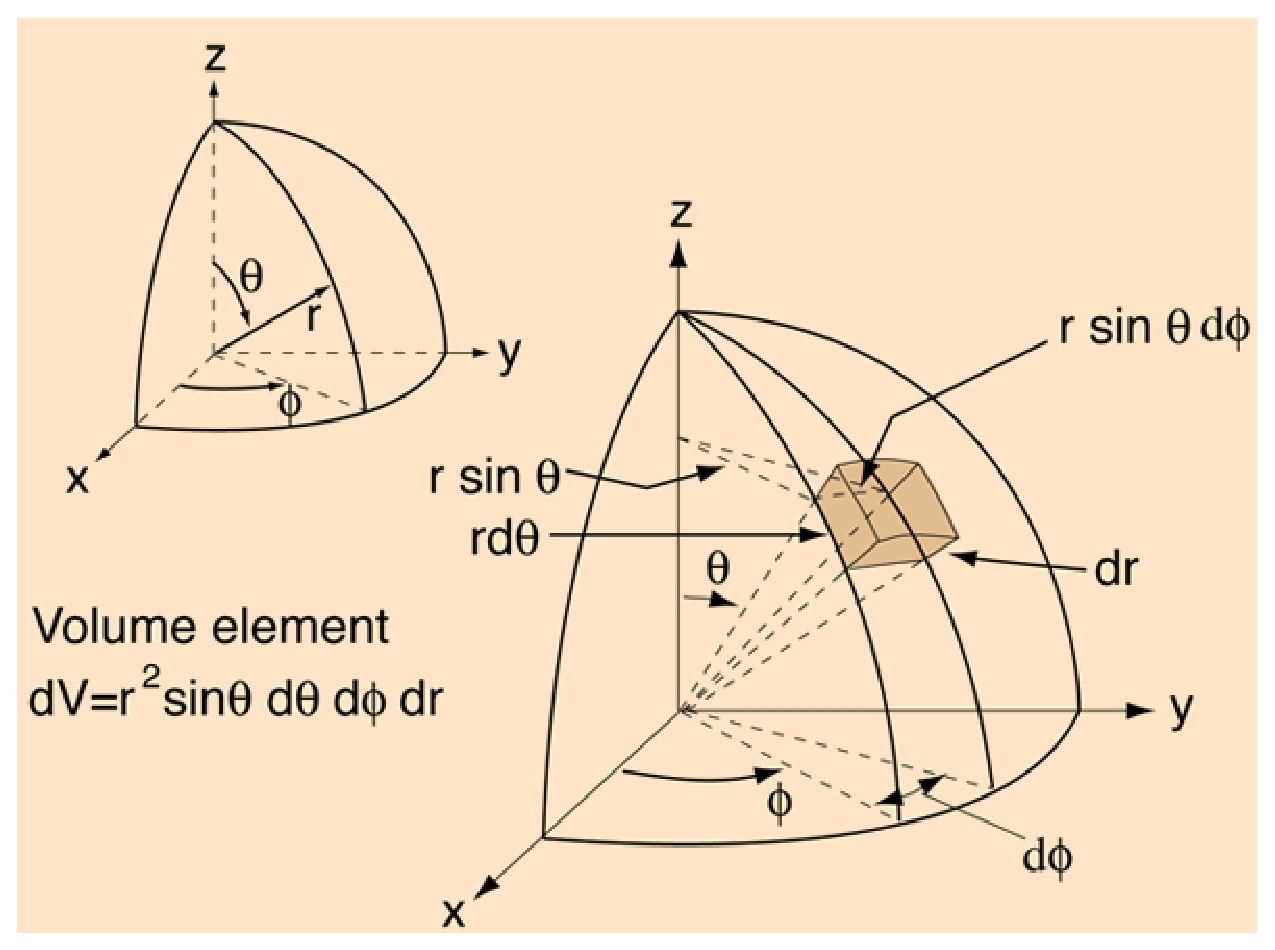
\includegraphics[height=5cm,
%     angle=0]{./images/spherical_coordinate.eps}}
  \centerline{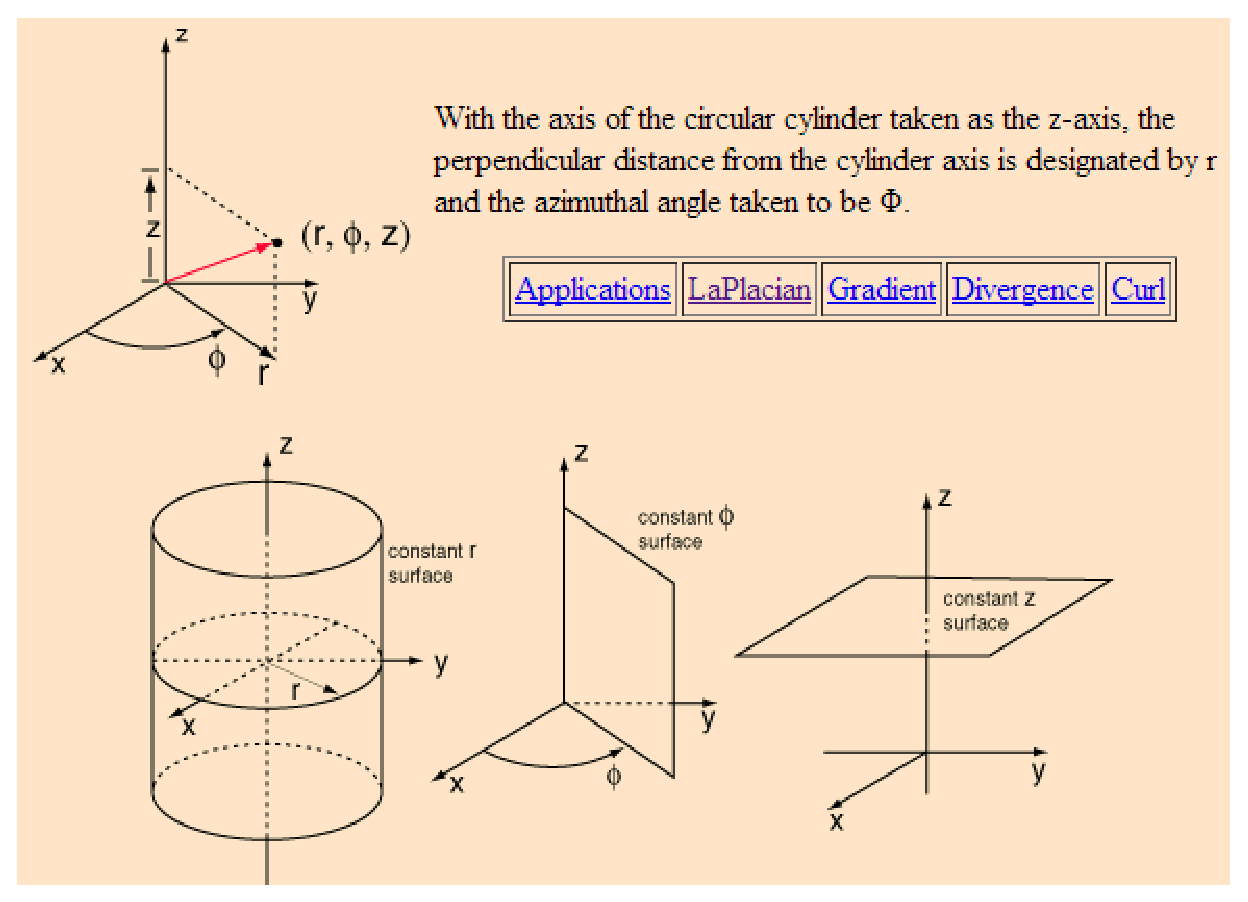
\includegraphics[height=5cm,
    angle=0]{./images/cylindrical_coordinate.eps}, 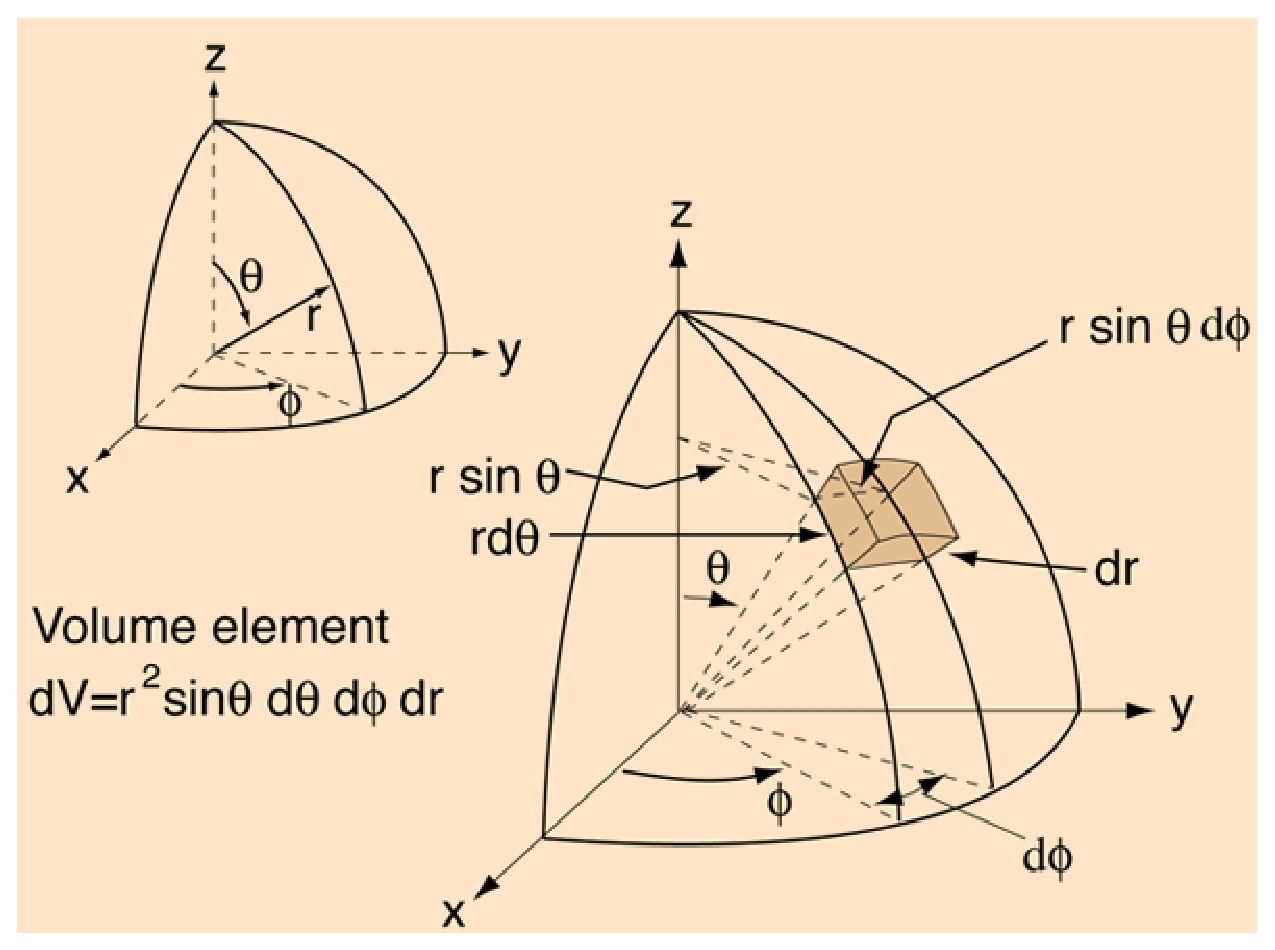
\includegraphics[height=5cm,
    angle=0]{./images/spherical_coordinate.eps}}
  \caption{(A) Cylindrical coordinates; (B) Spherical coordinates}
  \label{fig:coordinates}
\end{figure}


Under the assumption of {\it azimuthal symmetry}, i.e. the potential doesn't
vary in the $\phi	$ direction, i.e. $\partial V/\partial\phi = 0$. The
solution can be found using the method of separable variables, i.e. define a
functional form, i.e. the trial solution, and then separate the single equation
into two separate ODEs, one being the function of $r$ and the other being the
function of $\theta$. The unique solution is found when we apply the boundary
condition. 
\begin{equation}
V(r,\theta) = (A.r^l + Br^{-(l+1)})P_l.\cos(\theta)
\end{equation}
In Cartesian coordinates, the full solution is the sum of solution in the form
above
\begin{equation}
V(r,\theta) = \sum_{l=0}^\infty (A.r^l + Br^{-(l+1)})P_l.\cos(\theta)
\end{equation}
These are the second-order PDEs whose solutions give the correct form of the
electrical potential in the free space, satisfying the boundary condition. Given
the values at the boundary, the exact equations of the solution can be derived.

Example 2: consider a sphere of radius $R$ and of uniform charges: given the
charge density $\rho$, then the total charge in the sphere is 
\begin{equation}
Q = \frac{4}{3}\pi R^3\rho
\end{equation}
Combine the knowledge that at the same value
of $r$, all points have the same potential, so the derivative w.r.t $\theta$ and
$\phi$ must be zero. It means that eq.\ref{eq:spc} becomes the simpler form
\begin{equation}
\frac{\partial^2 V}{\partial r^2} + \frac{2}{r}\frac{\partial f}{\partial r} =
\frac{-\rho}{\varepsilon_o}
\end{equation}  
with the solution of a form $V=\frac{a}{r}+b$. We need to find $a,b$?

NOTE: Even though the region outside the sphere has no charge, there could still
be an electric field even though the charge density is zero. This electric field
originates from the charge that can be outside the region we're interested in.
We'll see how it works further.

To find the voltage, we need a reference point where we assume with zero
potential. If we put the reference point at infinite, then the sphere of charge
will look like a {\it point charge} at large distances, then the electric
potential (voltage) at any point in space (at a distance $r$ to the point
charge) produced by this point charge Q is given by the formula
\begin{equation}
V = \frac{Q}{4\pi r \varepsilon_o} = \frac{kQ}{r}
\end{equation}
with $k$ is Coulomb's constant
\begin{equation}
\begin{split}
k &= 8.987552\times 10^9 \text{Nm$^2$/C$^2$} \\
\varepsilon_o &= 8.854187817\times 10^{-12} \text{F/m}
\end{split}
\end{equation}
with (F=Farad, C=Coulomb).

For a point inside the sphere, then the solution (i.e. equation for voltage)
must have a term of order $r^2$ to give a constant on the left hand-size of the
equation, i.e. formula $V = cR^2+d$, then 
\begin{equation}
2c + 4c = \frac{-\rho}{\varepsilon_o}
\end{equation}
or $c=\frac{-\rho}{6\varepsilon_o}$. To find $d$, we use the boundary condition
(where $R=r$), then we substitute and get
\begin{equation}
d = \frac{Q}{4\pi\varepsilon_o r} + \frac{\rho r^2}{6\varepsilon_o}
\end{equation}
So, the full solution for the potential inside the sphere from Poisson equation
is
\begin{equation}
V = \frac{\rho}{6\varepsilon_o} \left[ R^2-r^2 \right] +
\frac{Q}{4\pi\varepsilon_o R}
\end{equation}

The general solution to Laplace equation in cylindrical coordinate
$(r,\phi,z)$ are
\begin{equation}
V(r,\phi,z) = \sum_{m=0}^\infty \left[ A_mJ_m(ks) + B_mN_m (ks) \right]
\left[ C_m\sin(m\phi) + D_m \cos(m\phi) \right] \left[ E_m\sinh(k z) + F_m
\cosh(k z) \right]
\end{equation}
The hard part is to determine the coefficients to satisfy the boundary
conditions.\footnote{\url{http://www.cord.edu/faculty/gealy/physics315/SepVarsCyl.pdf}}

\section{Potential -eccentric dipole in finite-length circular conducting
cylinder}

\citep{okada1956} used Laplace equation, with boundary condition of zero normal
derivative at the surface.  Compared with another point $P'$, the dipole of
source strength $I$ at location $P$ produces a potential
\begin{equation}
V = \frac{I}{4\pi\gamma r}
\end{equation}
with $r$ is the distance from the current source of position $P'(\rho',
\phi', z')$ to a point $P(\rho,\phi, z)$. 

\begin{figure}[hbt]
  \centerline{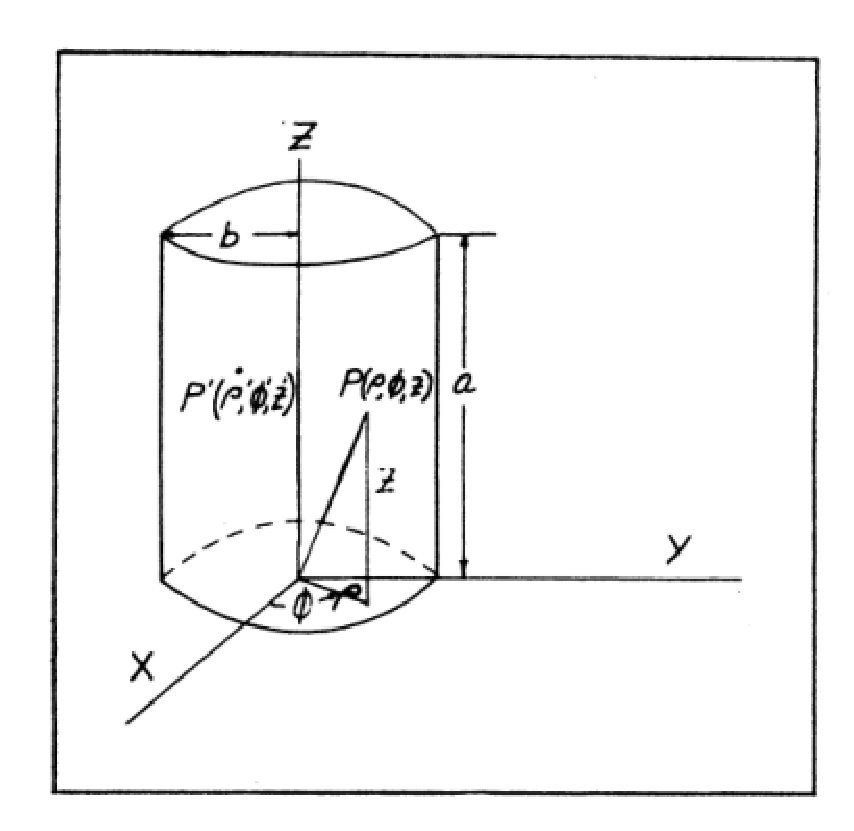
\includegraphics[height=5cm,
    angle=0]{./images/dipole_source.eps}}
  \caption{The circular cylinder and a z-oriented dipole source.
  When dipole is located on the axis of the cylinder, $\rho'=0$}
  \label{fig:dipole_source}
\end{figure}

{\bf Bessel functions} are widely used as they appear in the solution of Laplace
equation in the cylindrical coordinates. The potential is found by finding the
potential in each dimension separatedly, i.e. $V_r,V_\rho, V_\phi$. The inverse
distance $1/r$ can be expressed in terms of modified Bessel functions such that
the expression will converge for $\rho>\rho'$.
\begin{equation}
\frac{1}{r} = \frac{2}{\pi}\int^\infty_0	\cos(\lambda(z-z')) \sum^infty_{m=0}
(2-\delta_m^o) K_m(\lambda\rho) I_m(\lambda\rho') .\cos(m(\theta-\theta'))
d\lambda
\end{equation}
with $K_m, I_m$ are modified Bessel functions of order $m$; 
\begin{equation*}
\begin{array}{cc}
\delta_m^o=0 & 	m \ne 0	\\
\delta_m^o=1 & 	m = 0	
\end{array}
\end{equation*}


The potential produced by a current dipole oriented in the positive $z$
direction is obtained by partial differential of the point source potential
w.r.t. z, and replace the current strength $I$ by $-p_z$ with $p_z$ is the
dipole mement. 


\section{Potential - ecentric dipole in sphere or ellipsoid}

When the dipole is in a homogeneous conducting prolate spheroid, Legendre
equations are used instead \citep{yeh1957}. 
The prolate spheroid body has the semimajor axis $a$ and semiminor axis
$a\sqrt{1-e^2}$, with $0\le e \le 1$ as the eccentricity. The equation of the
surface is
\begin{equation}
\frac{\rho^2}{1-e^2} + z^2 = a^2
\end{equation}
using the cylindrical coordinate system $(z,\rho,\theta)$ which is chosen so
that the spheroid is coaxial with the $z$-axis.


\section{ECG - Heart activity}

Solving the problem is challenging as we need to calculate the complete
potential distribution on an irregularly (torso) shaped external surface, based
on the arbitrary source distribution (the heart, or the generator) in a medium
containing regions of different conductivity (the human body, the bath). Also,
it's subjected to boundary condition that the generated curernts be tangible to
the external boundary and continuous through all internal interfaces between
media of different conductivity, i.e. the normal component of the electric field
vanishes at the external boundary (the body skin), and the electric field is
refracted at the interfaces.


\section{ECG database}

ECG is an inexpensive, noninvasive technique to record heart's electrical
activity. Holter, in 1961, developed the device that can continuously record
the ECG. Holter monitor is a portable device to record ECG signal continuously
24 or 48 hrs.  Even though the recorded data are plentiful, there are only a few
database available for common researches
\begin{enumerate}
  \item THEW project: Sect.\ref{sec:THEW}
  
  \item MIT-BIH Arrhythmia Database: Sect.\ref{sec:MIT-BIH_Arrhythmias}
  \item  AHA Database for Evaluation of Ventricular Arrhythmias Detectors:
  created from 1977-1985
  \item European ST-T Database
\end{enumerate}
This will facilitates the algorithm development for automatic arrhythmia
analysis algorithms.

\subsection{MIT-BIH Arrhythmias Database}
\label{sec:MIT-BIH_Arrhythmias}

Data are selected as 48 recordings, each is a half-hour excerpts of 2-channel,
24-hour ECG recording  from 47 subjects, i.e. measured from 25 men (32-89 years)
and 22 women (23-89  years), with 60\% are inpatients during the year 1975 to
1979  \citep{moody2001}. The 48 records are put into 100 series and 200 series.
The  100 series (23 records) data are randomly selected from over 4000 Holter
tapes, and the 200 series (25 records) data are selected to include examples  of
uncommon, but clinically important arrhythmias. With 47 subjects and 48 
records, it means 2 records (201 an 202) are from the same subjects.
  An example: Fig.\ref{fig:ECG_10sec} from record 205 that display VT.  
\url{http://ecg.mit.edu/george/publications/mitdb-embs-2001.pdf}
    
\begin{figure}[hbt]
 \centerline{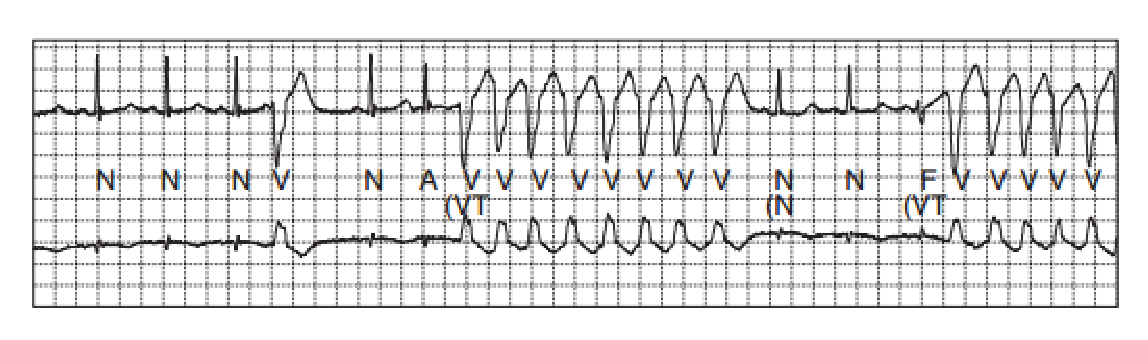
\includegraphics[height=7cm]{./images/ECG_10sec.eps}}
 \caption{10 second read from record 205 of MIT-BIH Arrhythmia Database. Rhythm
 annotation (N=normal, VT = ventricular tachycardia)}
\label{fig:ECG_10sec}
\end{figure}

How the signals are annotated in MIT-BIH Arrhythmias Data? 
\begin{itemize}
  \item Device: Del Mar Avionics model 445 two-channel reel-to-reel Holter
  recorders. This analog signal is then playbacked using Del
Mar Avionics model 660 playback unit to digitize the data. The digitization
rate: 360 samples per second per channel. During digitalization, a passband of
0.1 Hz to 100 Hz relative to real time was used to filter, e.g. most 60 Hz noise
in the recording was introduced during playback. This noise appear at 30 Hz or
multiple of 30 Hz.
  
  \item The signal are then annotated using a simple slope-sensitive QRS
  detector. The cardiologists added rhythm and signal quality labels. 
  
NOTE: Six of the 48 records (from the original MIT-BIH Arrhythmias Data) contain
a total of 33 beats remain unclassified, as the cardiologists didn't reach the
agreement on the beat type (normal or abnormal).
\end{itemize}

From 1980s, more data were added. In 1989, seven other ECG database was added
along with MIT-BIH Arrhythmias database. In 1999, PhysioNet project was created
(\url{http://www.physionet.org/}), a Web-based resource for research on complex
physiologic signals.


\subsection{THEW project}
\label{sec:THEW}

Telemetric and Holter ECG Warehouse (THEW) is the effort to provide resources
(data + tools) to conduct ECG-related researches [NOTE: Holter is the name of
the battery-operated portable device to measure ECG continuously for 24-48
hours]. It currently hosts more than 3,700 digital 24-Holter ECG recordings from
13 independent studies. We can use the data to develop the ECG-based
technologies.

\begin{framed}
Cardiac safety is still the major issue in drug and device testing. It was
estimated that as many as 86\% of all new chemical entities (NCE) tested in
pharmaceutical development show specific inhibitory effect, i.e. prolong the
ventricular repolarization, which in some cases can lead to Torsades de Pointes
(TdPs) and potentially SCD.

Tools currently being used was developed since the last century. Thus, there is
an increasing demand to develop new tools.

Holter device is being used like a standard ECG. It records the electrical
signals via a number of electrodes attached to the chest (put near the bone to
minimize artifacts from muscular activity). The number of electrodes are in the
range 3-8.
\end{framed}


\section{ISHNE Holter Standard Output File format}
\label{sec:ISHNE_Holter-FileFormat}


Efforts to develop a standard file format interchangeable between
Holter manufacturers started in 1997. Each data has 2 file: ECG file (.ecg) and
annotation file (.ann)
\begin{verbatim}
S1123.ann
S1123.ecg
\end{verbatim}
The first version is limited to ECG standardization, but not yet annotation
file \citep{zareba1998}. \url{http://thew-project.org/THEWFileFormat.htm}

\begin{Verbatim}
char * cstr = mxArrayToString(prhs[0]);
std::ifstream file_id(cstr, std::ifstream::binary);

char magic[9];
file_id.read(magic, sizeof(magic)-1);

\end{Verbatim}
\begin{enumerate}
  \item The very beginning part of the file is the 'magic' number: which is a
  string of 8 characters: ``ISHNE1.0'', i.e .the string length should be 9 to
  include the string-terminator.
\begin{verbatim}

\end{verbatim}
\end{enumerate}

The ECG file is organized with a header, followed by a larger data block
(containing all ECG digital samples). 
The header structure
\begin{verbatim}
/* short int = 1byte
   long int  = 4
   unsinged int = 2
   char         = 1
*/
struct ishne_t {
  int32_t Var_length_block_size;
  int32_t Sample_size_ECG;
  int32_t Offset_var_length_block;
  int32_t Offset_ECG_block;
  int8_t  File_version;
  char    First_name[40];
  char    Last_name[40];
  char    ID[20];
  int8_t  Sex;
  int8_t  Race;
  int8_t  Birth_date[3];
  int8_t  Record_date[3];
  int8_t  File_date[3];
  int8_t  Start_time[3];
  int8_t  Num_leads;
  int8_t  Lead_spec[12];
  int8_t  Lead_qual[12];
  int8_t  Resolution[12];
  int8_t  Pacemaker;
  char    Recorder[40];
  int8_t  Sampling_rate;
  char    Proprietary[80];
  char    Copyright[80];
  char    Reserved[80];
}
\end{verbatim}


\section{Algorithms to analyze ECG data}



\section{Cardiac output}
\label{sec:cardiac-output}

\url{https://en.wikipedia.org/wiki/Cardiac_output}

\section{Cardiac hypertrophy}
\label{sec:cardiac-hypertrophy}

\begin{framed}
Cardiac hypertrophy is defined by an increase in heart size and/or myofibrillar
volume without a change in myocyte number (i.e. no myocyte cellular
proliferation), which occurs in response to both physiological and
pathophysiological stimulation. 

While cardiac hypertrophy is considered as a normal change to the heart in
response to normal ventricular wall stress, the sustained hypertrophy is
correlated with the incidence and mortality in heart disease, with the first
step is the progression to congestive heart failure (CHF) \citep{levy1990}. 

Cardiac hypertrophy is also a risk factor for cardiac arrhythmia and sudden
cardiac death due to prolonged APD. The prolonged APD is the result of the
down-regulation of $\K$ currents ($I_\to$). The mechanism of reduction of
$I_\to$ in heart failure, i.e. change in Kv4.2 mRNA level decrease 30\%
\citep{kaab1998} (Sect.\ref{sec:mRNA-level-2-protein-expressio}).

\end{framed}

Using Csa/FK506 to test the role of Calcineurin (Sect.\ref{sec:calcineurin}),
there are 'yes' and 'no' for the fact that Calcineurin as an important
transducing factor in cardiac hypertrophy. The reason for these controversal
results can be explained by the side-effect of using high dose of Csa/FK506 that
can alter SR $\Ca$ release through RyR or other non-specific leakage, and Csa
also inhibit Na/K-ATPase, etc.

In cardiac, there are 4 members NFATc1-NFATc4 which are activated only by
calcineurin. The amount and timing for the nuclear translocation of NFAT are
directly proportional to the degree of calcineurin activation {\it in vivo}
\citep{hogan2003}. However, measuring NFAT nuclear translocation in intact cell
is often not possible so far.


Cardiac-specific MCIP1 overexpressing transgenic mice demonstrated no
hypertrophy under isoproterenol infusion, treadmill running, pressure overload,
etc. (review: \citep{wilkins2002cac}). Interestingly, the first known feedback
regulator of calcineurin activity was found with MCIP1 \citep{yang2000}. The
third introns of human MCIP1 gene contains a cluster of 15 consensus NFAT
binding sites, i.e. NFAT can regulat MCIP1 expression level and MCIP1 inhibit
Calcineurin which activate NFAT.
